\subsection{Instructor}

Instructors have a lot of responsibility when it comes to selecting students to be TAs for their classes.
They are usually given the final say on all selections, so the power really rests in their hands.
In our project, we focused on letting them decide students they favor or disfavor and selecting the necessary skills needed for their sections.

\begin{figure}[!htb]
  \centering
  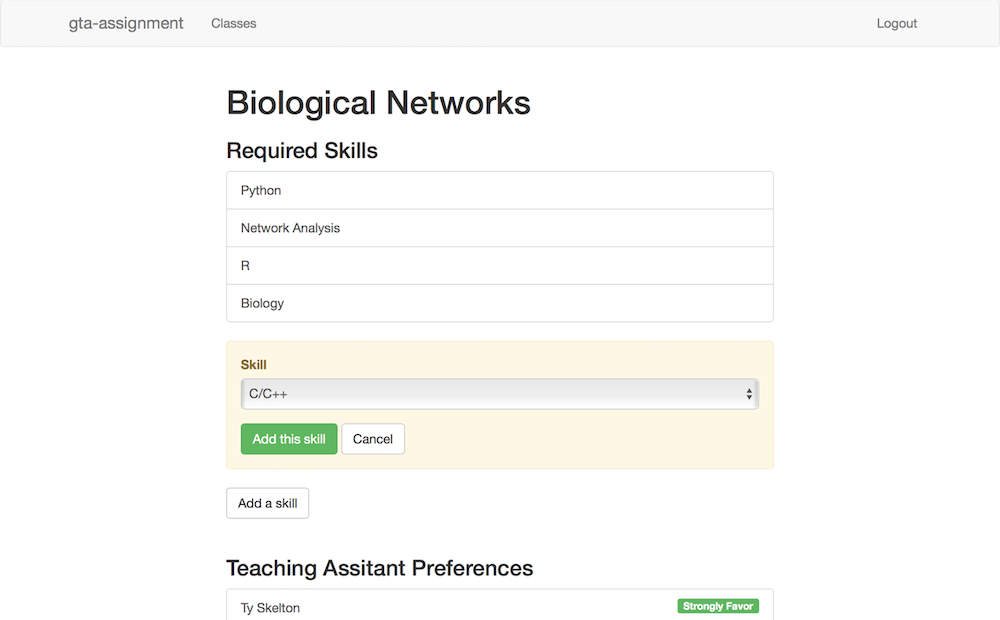
\includegraphics[width=0.75\linewidth]{images/instructor-section-design.png}
  \caption{Mock Instructor Sections Page}\label{instructor-section-design}
\end{figure}

\begin{figure}[!htb]
  \centering
  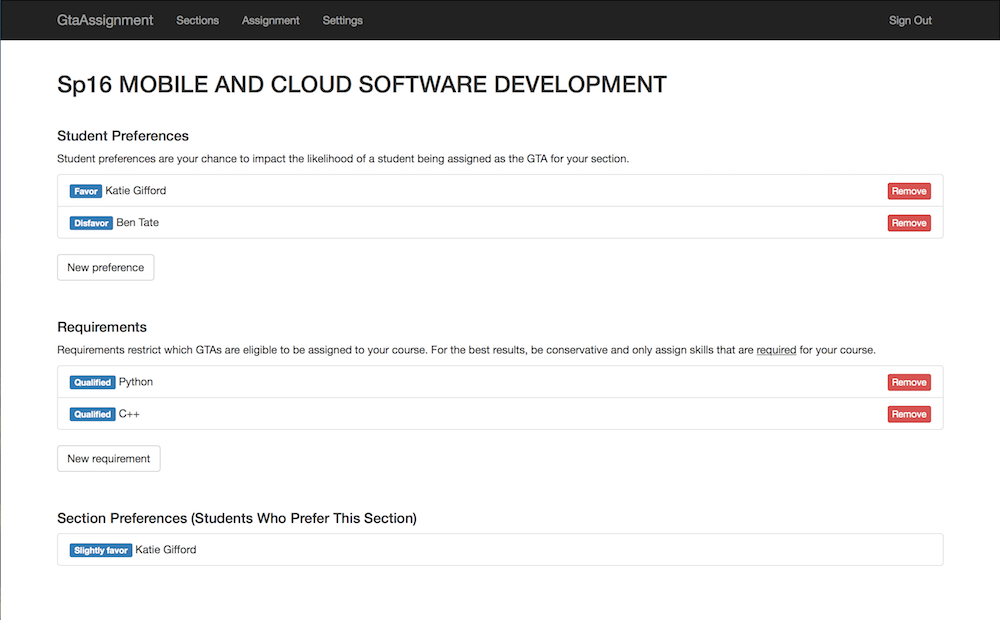
\includegraphics[width=0.75\linewidth]{images/instructor-section-beta.png}
  \caption{Release Instructor Sections Page}\label{instructor-section-beta}
\end{figure}

% \begin{figure}[!htb]
%   \centering
%   \minipage{0.5\textwidth}
%     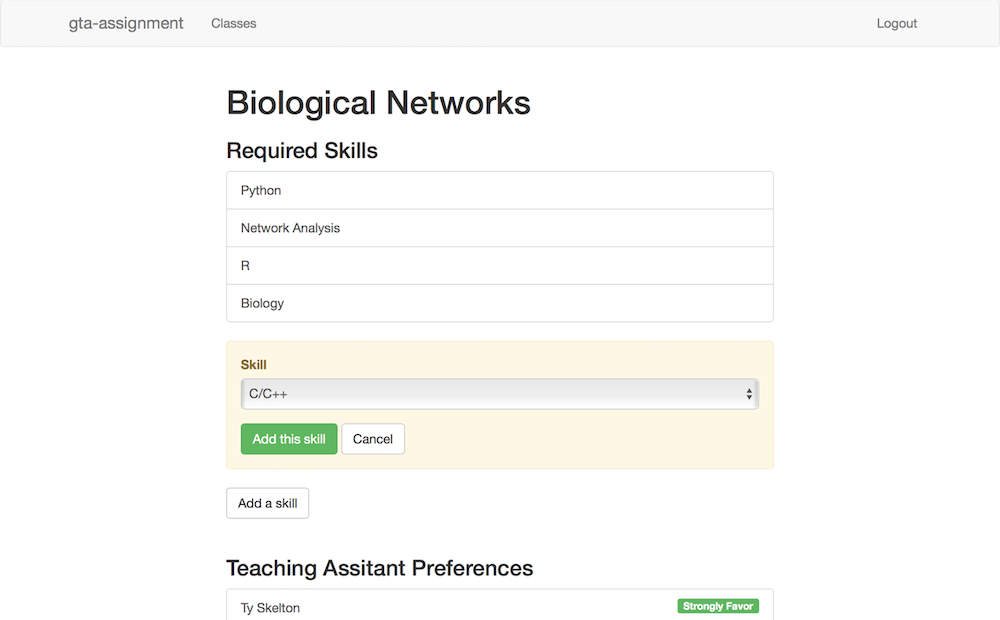
\includegraphics[width=\linewidth]{images/instructor-section-design.png}
%     \caption{Mock Instructor Sections Page}\label{instructor-section-design}
%   \endminipage\hfill
%   \minipage{0.5\textwidth}
%     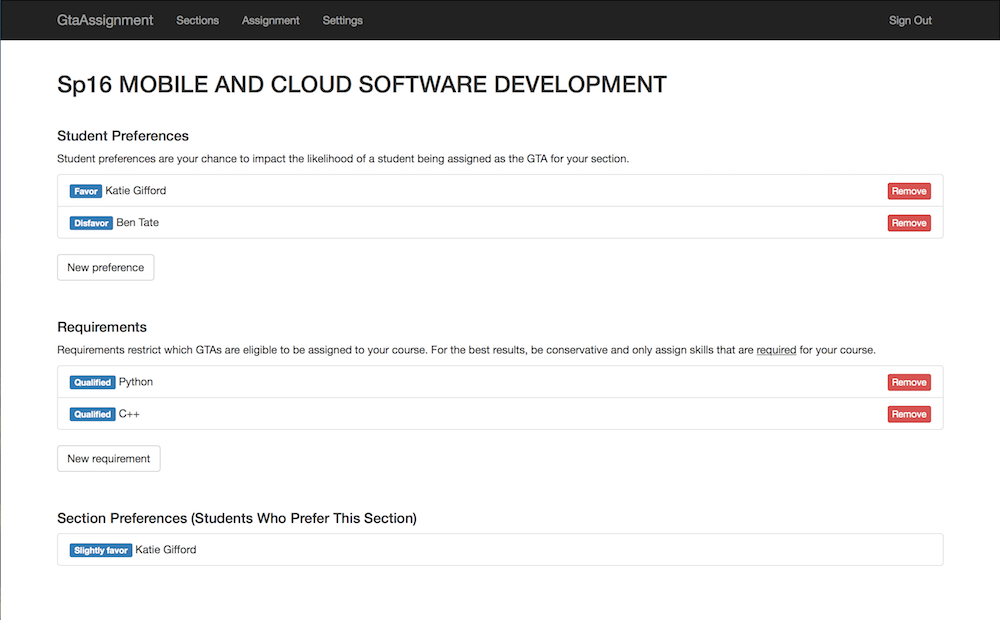
\includegraphics[width=\linewidth]{images/instructor-section-beta.png}
%     \caption{Release Instructor Sections Page}\label{instructor-section-beta}
%   \endminipage\hfill
% \end{figure}

As you can see, we split the classes into sections.
Many instructors are teaching multiple classes each with its own section number.
This allows them to associate experiences and preferences on each of the sections that they teach.
It is always kept up to date because of our class scrapper.
Once you press the section you will be brought to a detailed section interface shown in Figures \ref{instructor-section-design} and \ref{instructor-section-beta}.

Each section has its own required skills which can be set by the instructor.
These are hard constraints when it comes to the ILP, so choosing the correct skills is a important job of the instructor.
The new preference button looks a lot like the add skill page for the students, it brings up a list of students where you can set a preference based on the same range of values as the students: disfavor up to favor.
Both are fully implemented and can be seen in our video presentation.
